In this section, we describe the software architecture of the HydroTracker system, which monitors the status of multiple sensor nodes in real time. The application is composed of two primary components:
\begin{itemize}
    \item A background thread that reads and processes incoming serial data.
    \item A user interface that visualizes node states in real-time using colored labels.
\end{itemize}

\subsection{Reading from the Serial}

Serial communication is handled by the \texttt{SerialReaderThread} class, which operates in a separate background thread to prevent GUI blocking. Its main functionality is found in the \texttt{read\_serial()} method. The thread checks if data is available (\texttt{in\_waiting > 0}), reads and decodes the incoming string, and logs it. If the message follows the format \texttt{Node<id> - State:<STATE>}, the node ID and state are extracted. This call delegates the responsibility of updating the GUI to the main application \texttt{HydrotrackerMonitor}.

\subsection{Data Processing}
Once a valid line is received, it is parsed into two key components:
\begin{itemize}
    \item \texttt{node\_id}: the identifier of the node
    \item \texttt{state}: the reported status (e.g., "EMPTY", "NOTEMPTY", or "NOTEXIST")
\end{itemize}
After extracting these, the GUI is updated only if the state has changed. Each node has an entry in a dictionary \texttt{node\_states} that keeps track of its most recent state. This structure enables efficient state tracking and minimizes unnecessary GUI updates.

The following snippet illustrates the logic used to parse incoming serial messages and trigger GUI updates accordingly:
\begin{lstlisting}[language=Python, caption={Serial data parsing and GUI update}]
if self.serial_conn.in_waiting > 0:
    # Read incoming serial line
    line = self.serial_conn.readline().decode('utf-8').strip()
    
    # Check if it matches the expected format
    if line.startswith("Node") and " - State: " in line:
        before, _, after = line.partition(" - State:")
        node_id_str = before.replace("Node", "").strip()
        state = after.strip()
        
        # If valid node ID, update the GUI
        if node_id_str.isdigit():
            self.app.update_node_state(int(node_id_str), state)
\end{lstlisting}

\subsection{User Interface}
The GUI is created using Python's \texttt{tkinter} module and is managed by the \texttt{HydrotrackerMonitor} class. For each detected node, a label is dynamically added with the method \texttt{create\_gui\_label(node\_id)}. Each label changes its color and text based on the node's current state. This is managed in the \texttt{update\_gui\_loop()} method, which periodically refreshes the display.
The following listing illustrates this logic:

\begin{lstlisting}[language=Python, caption={GUI update and label coloring based on node state}]
def update_gui_loop(self):
    for node_id, state in self.node_states.items():
        label = self.labels[node_id]
        label.config(text=f"Node {node_id}: {state}") 

        if state == "EMPTY":
            label.config(bg="#e74c3c", fg="white")  # red
        elif state == "NOTEMPTY":
            label.config(bg="#2ecc71", fg="white")  # green
        elif state == "NOTEXIST":
            label.config(bg="#7f8c8d", fg="white")  # gray
        else:
            label.config(bg="#bdc3c7", fg="black")  # default

    self.root.after(UPDATE_INTERVAL, self.update_gui_loop)
\end{lstlisting}

The following figures present the graphical user interface (GUI) of the HydroTracker system during runtime. The interface dynamically updates based on real-time input from the sensor nodes. Each label represents a specific node and changes color and text to reflect its current state. The visual encoding allows the user to quickly identify which tables require attention.


\begin{figure}[H]
    \centering
    \begin{subfigure}[b]{0.4\linewidth}
        \centering
        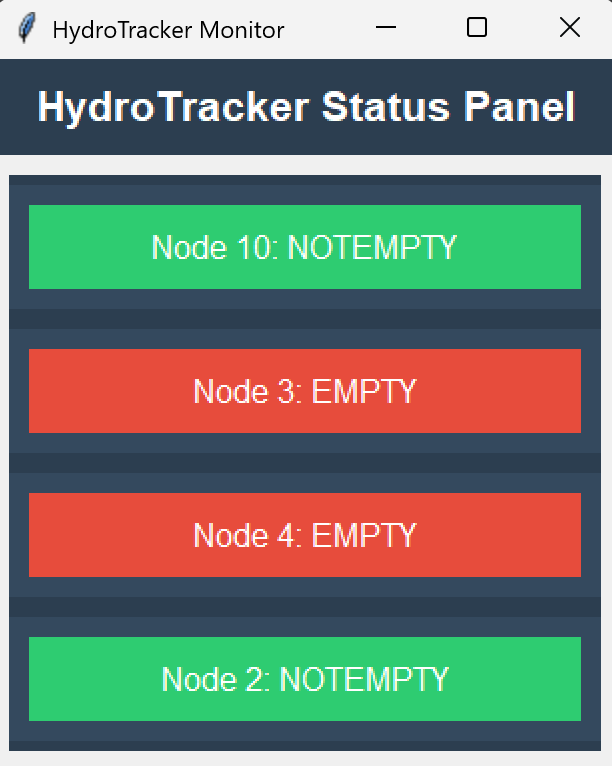
\includegraphics[width=\linewidth]{gui_images/gui_screenshot_1.png}
        \caption{Instance of GUI}
        \label{fig:subfig1}
    \end{subfigure}
    \hfill
    \begin{subfigure}[b]{0.4\linewidth}
        \centering
        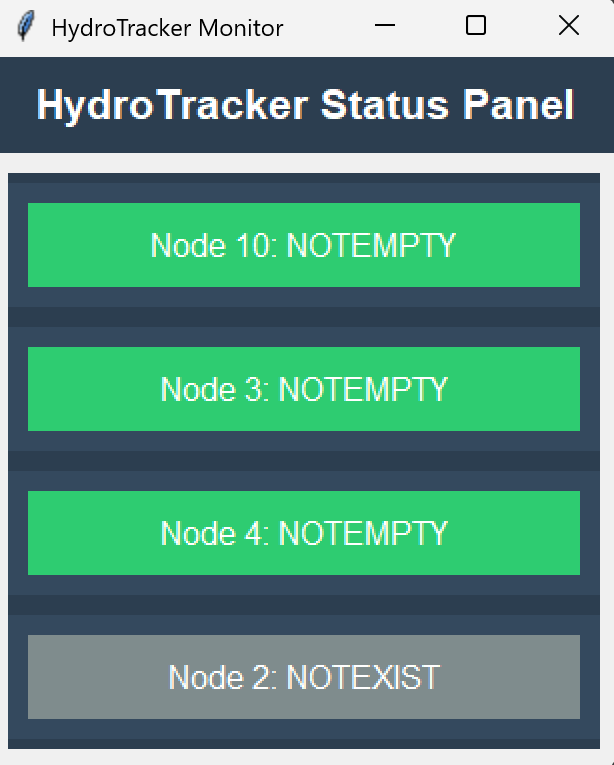
\includegraphics[width=\linewidth]{gui_images/gui_screenshot_2.png}
        \caption{Instance for GUI}
        \label{fig:subfig2}
    \end{subfigure}
\caption{Graphical interface of HydroTracker displaying node states. Left: all nodes active. Right: one node marked as NOTEXIST.}
    \label{fig:combined}
\end{figure}

%\begin{figure}[H]
    %\centering
    %\includegraphics[width=0.3\linewidth]%{gui_images/flowchart_datapro.png}
    %\caption{Enter Caption}
    %\label{fig:enter-label}
%\end{figure}